\section{Verlustbehaftete Kompression von volumetrischen Punkten}
Wissenschaftliche Simulationen produzieren grosse Mengen an Daten. Es werden Schwingungen, Flugbahnen, Flüsse, Kraftfelder etc. als Linien im dreidimensionalen Raum visualisieren. Die Linien können als Folge von volumetrischen Punkten dargestellt werden. Die Datenmenge ist oft zu gross als dass sie in sinnvoller Zeit über eine Internetverbindung übertragen werden können. Deshalb soll im rahmen dieser Arbeit eine verlustbehaftete Kompression entwickelt werden, welche die Datenübertragung ermöglicht.\\
[\baselineskip]
Im Rahmen dieses Projekts müssen Daten von Magnetfeldlinien der Sonne über eine Internetverbindung zum JHelioviewer übertragen werden. Der JHelioviewer ist eine Applikation zur visualisierung von Satellitenmessdaten und Simulationen der Sonne. Die Applikation wird von der ESA und der FHNW entwickelt. Die Abbildung \ref{einleitung::feldlinien} zeigt eine Visualisierung des JHelioviewers.\\
\begin{figure}[!htbp]
\center
	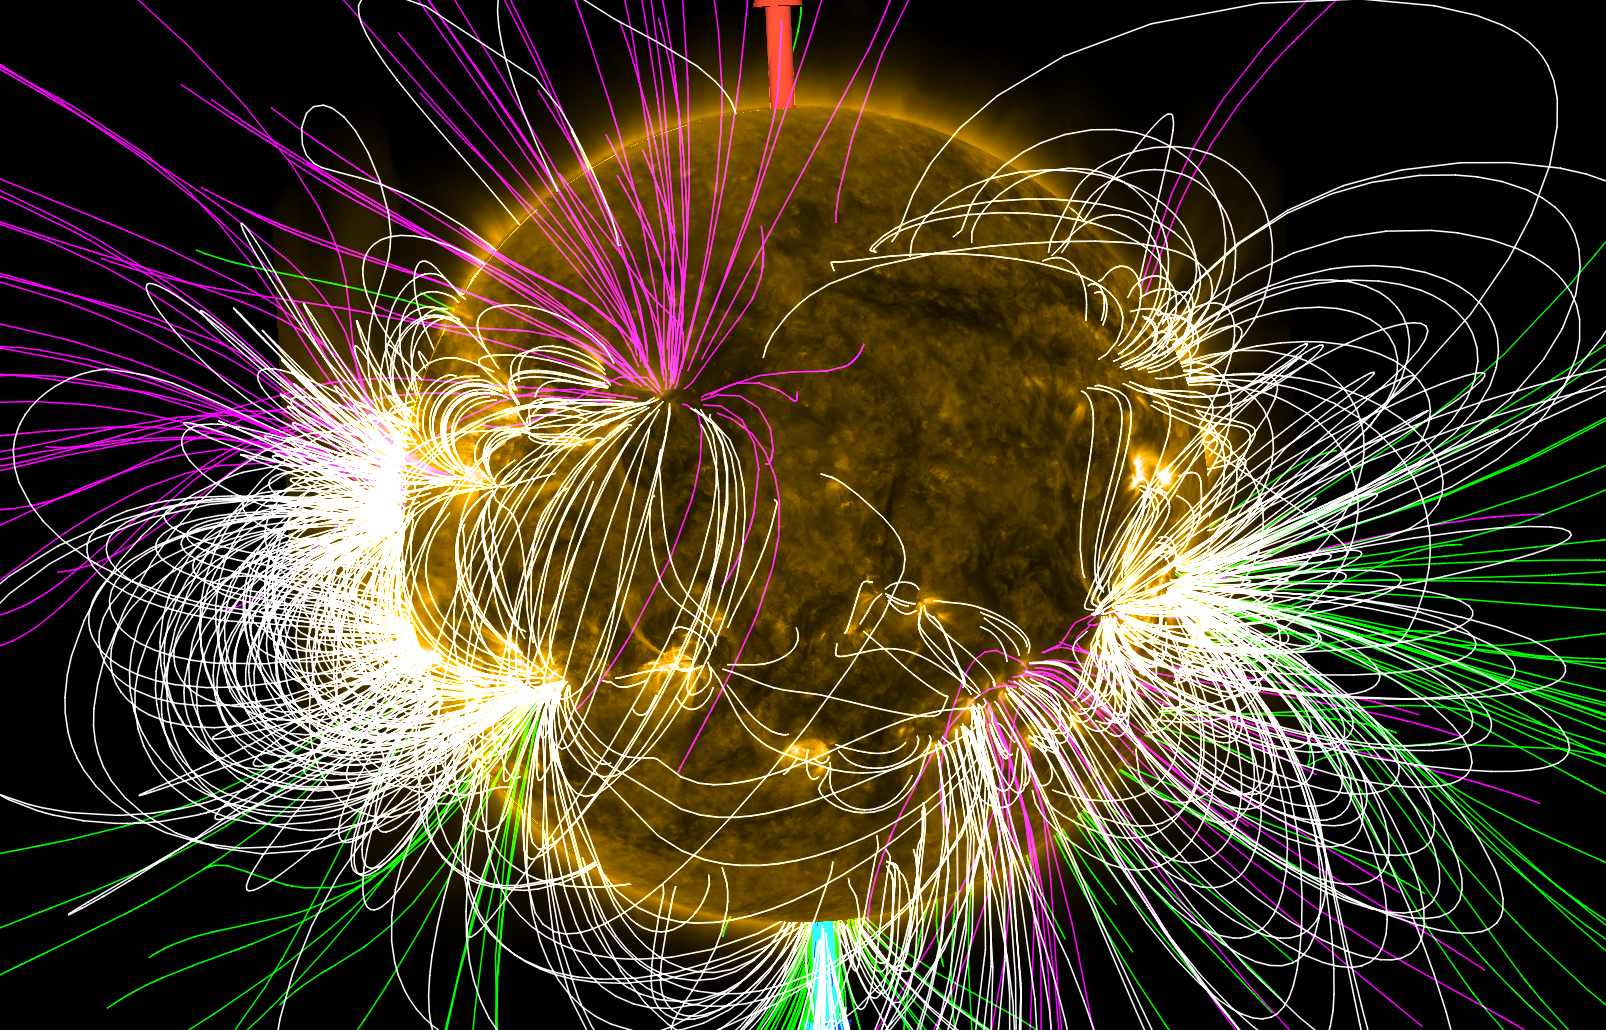
\includegraphics[width=0.8\textwidth,height=8cm,keepaspectratio]{./pictures/einleitung/fieldLines.png}
	\caption{Visualisierung der Feldlinien im JHelioviewer}
	\label{einleitung::feldlinien}
\end{figure}
Es wurde eine Aufnahme der Sonnenoberfläche zusammen mit drei Arten von Feldlinien visualisiert: Linien, die auf der Sonne starten und wieder auf der Sonne landen, auf der Sonne starten und ins Weltall führen oder vom Weltall auf der Sonne landen. Die weissen Feldlinien repräsentieren ''Sonne zu Sonne´´, die Grünen ''Sonne zu Weltall´´ und die Violetten ''Weltall zu Sonne´´.\\
[\baselineskip]
Der JHelioviewer visualisiert mehrere Messungen oder Simulationen in Abfolge. Ziel ist es, möglichst schnell die Mess- und Simulationsdaten abzuspielen, sodass der Benutzer eine flüssige Animation erhält. Pro Simulation werden etwa 1.5 MiByte and Feldliniendaten generiert. Bei einer Visualisierung muss der JHelioviewer die Feldlinien- und andere Daten zur Laufzeit herunterladen.
Internetverbindung wird stark beansprucht und Benutzer muss auf Frames warten.

Potential Field Source Surface (PFSS) Simulation, welche aus Messungen der Sonnenoberfläche die Magnetfeldlinien extrapoliert, produziert pro Aufnahme etwa 1.5 Mibyte an Daten. welche zur Laufzeit über eine Internetverbindung heruntergeladen wird. Mit einer verlustbehafteten Kompression soll die zu übertragende Datenmenge deutlich verkleinert werden.

Resultate

Wo was beschrieben wird.




 